% --------------------------------------------------------------
% This is all preamble stuff that you don't have to worry about.
% Head down to where it says "Start here"
% --------------------------------------------------------------
 
\documentclass[12pt]{article}
 
\usepackage[margin=0.8in]{geometry} 
\usepackage{hyperref}
\usepackage{url}
\usepackage{xcolor}
\usepackage{array}

\usepackage{dashrule}
\usepackage{multirow}

\usepackage{amsmath,amsthm,amssymb}
\usepackage{turnstile}
\usepackage{mathtools}
\usepackage{bm}
\DeclarePairedDelimiter\ceil{\lceil}{\rceil}

\usepackage{algorithm}
\usepackage[noend]{algpseudocode}
\usepackage{pifont}

\usepackage{graphicx}
\usepackage{subfigure}
\graphicspath{{images/}}    %change appropriately if required

\newcommand{\x}{\bm{x}}
\newcommand{\bvec}{\bm{b}}
\newcommand{\norm}[1]{\left\lVert#1\right\rVert}
\renewcommand{\algorithmicforall}{\textbf{for each}}
\newlength\myindent % define a new length \myindent
\setlength\myindent{6em} % assign the length 2em to \myindet
\newcommand\bindent{%
  \begingroup % starts a group (to keep changes local)
  \setlength{\itemindent}{\myindent} % set itemindent (algorithmic internally uses a list) to the value of \mylength
  \addtolength{\algorithmicindent}{\myindent} % adds \mylength to the default indentation used by algorithmic
}
\newcommand\eindent{\endgroup} % closes a group

\newenvironment{theorem}[2][Theorem]{\begin{trivlist}
\item[\hskip \labelsep {\bfseries #1}\hskip \labelsep {\bfseries #2.}]}{\end{trivlist}}
\newenvironment{lemma}[2][Lemma]{\begin{trivlist}
\item[\hskip \labelsep {\bfseries #1}\hskip \labelsep {\bfseries #2.}]}{\end{trivlist}}
\newenvironment{exercise}[2][Exercise]{\begin{trivlist}
\item[\hskip \labelsep {\bfseries #1}\hskip \labelsep {\bfseries #2.}]}{\end{trivlist}}
\newenvironment{problem}[2][Problem]{\begin{trivlist}
\item[\hskip \labelsep {\bfseries #1}\hskip \labelsep {\bfseries #2.}]}{\end{trivlist}}
\newenvironment{question}[2][Question]{\begin{trivlist}
\item[\hskip \labelsep {\bfseries #1}\hskip \labelsep {\bfseries #2.}]}{\end{trivlist}}
\newenvironment{prt}[2][Part]{\begin{trivlist}
\item[\hskip \labelsep {\bfseries #1}\hskip \labelsep {\bfseries #2.}]}{\end{trivlist}}
\newenvironment{corollary}[2][Corollary]{\begin{trivlist}
\item[\hskip \labelsep {\bfseries #1}\hskip \labelsep {\bfseries #2.}]}{\end{trivlist}}
\newenvironment{solution}[1][Solution]{\begin{trivlist}
\item[\hskip \labelsep {\bfseries \underline{#1}.} ]}{\end{trivlist}}
\newenvironment{definition}[1][Definition]{\begin{trivlist}
\item[\hskip \labelsep {\bfseries #1.}]}{\end{trivlist}}
 \hypersetup{%
  colorlinks=true,% hyperlinks will be coloured
  linkcolor=blue,% hyperlink text will be green
  linkbordercolor=red,% hyperlink border will be red
}

\begin{document}
 
% --------------------------------------------------------------
%                         Start here
% --------------------------------------------------------------
 
\title{Assignment-1\\ %change
\large{CS 388: Natural Language Processing} %Change
\author{Shobhit Chaurasia {\small(sc52987)}} \\
%replace with your name
% \small{(uteid: sc52987 | email: \href{mailto:shobhit@utexas.edu}{shobhit@utexas.edu})}
\date{}
} %if necessary, replace with your course title
 
\maketitle
\hrule
\begin{table}[h]
\caption{Bigram Model}
\label{table:forward}
\centering
  \begin{tabular}{|c|c|c|c|c|}
  \hline
  {\bf Dataset} & \multicolumn{2}{|c|}{{\bf Training}} & \multicolumn{2}{|c|}{{\bf Testing}} \\
  \hline 
  & Perplexity & Word Perplexity & Perplexity & Word Perplexity \\
  \hline
  atis & 9.0 & 10.6 & 19.3 & 24.0 \\
  wsj & 74.3 & 88.9 & 219.7 & 275.1 \\
  brown & 93.5 & 113.3 & 231.3 & 310.7 \\
  \hline
  \end{tabular}
\end{table}

\begin{table}[h]
\caption{Backward Bigram Model}
\label{table:backward}
\centering
  \begin{tabular}{|c|c|c|c|c|}
  \hline
  {\bf Dataset} & \multicolumn{2}{|c|}{{\bf Training}} & \multicolumn{2}{|c|}{{\bf Testing}} \\
  \hline 
  & Perplexity & Word Perplexity & Perplexity & Word Perplexity \\
  \hline
  atis & 9.0 & 11.6 & 19.4 & 27.2 \\
  wsj & 74.3 & 86.7 & 219.5 & 266.3 \\
  brown & 93.5 & 110.8 & 231.2 & 299.7 \\
  \hline
  \end{tabular}
\end{table}

\begin{table}[h]
\caption{Bidirectional Bigram Model}
\label{table:bidirectional}
\centering
  \begin{tabular}{|c|c|c|}
  \hline
  {\bf Dataset} & {\bf Training} & {\bf Testing} \\
  \hline 
  & Word Perplexity &  Word Perplexity \\
  \hline
  atis & 7.2 & 12.7 \\
  wsj & 46.5 & 126.1 \\
  brown & 61.5 & 167.5 \\
  \hline
  \end{tabular}
\end{table}

Table. \ref{table:forward}, \ref{table:backward}, and \ref{table:bidirectional} show the perplexity and word perplexity values for Bigram, Backward Bigram, and Bidirectional Bigram model respectively.

Before performing experiments, my prior belief was that the Bigram and the Backward Bigram models should not have significant difference in their performance on modeling English language, although, I expected the Backward Bigram model to be slightly worse than the Bigram model. This belief was stemmed from the notion that the English language is written from left to right, and hence, should be modeled better in the same direction. This reasoning seems to firmly advocate the notion that the performance of the Backward model should be drastically poor. However, this is not the case, since our measure of performance is perplexity (or word perplexity), which is intimately tied to a model, and measures how well does a system trained in a specific way (using a particular modeling technique) fare on sentences treated as having been generated using the same modeling technique. In simpler terms, perplexity measures how well can a model that generates sentences from, say, right-to-left fare on sentences if that are also viewed as being generated from right-to-left. Hence, one could reasonably expect a poor performance from the Backward Bigram model on generation of sentences from left-to-right, but it should perform reasonably well on generating sentences from right-to-left. With insignificant differences in word perplexities for Bigram and Backward Bigram models, the experiments back this reasoning.

Since the Bidirectional model captures both the right and the left context of a token, it should be plagued by comparatively fewer (and less grave) ambiguities, since we do not expect many words to correctly fill a gap between two words, except, for example, nouns surrounded by articles and verbs (e.g., the \underline{\hspace{0.5cm}} flies). The experiments seem to support our belief, with word perplexities for the Bidirectional model being nearly half of those of both the Bigram and the Backward Bigram model. The reduction in the \texttt{atis} dataset is not that drastic, probably because it is a fairly small dataset, on which the performance of any language model should be taken with a grain of salt. An interesting observation for the \texttt{atis} dataset is that the word perplexity for the test set for Bidirectional Bigram model is (slightly) higher than the other two models. A plausible reason behind this could be the presence of unusually high number of nouns (names of cities/countries) surrounded by prepositions (e.g. flight from \underline{\hspace{0.5cm}} to). Sentences like these can significantly `perplex' the Bidirectional model because of the huge list of possible tokens (city names) that can fill the blank. However, the Bigram and the Backward bigram models might also be plagued by this artifact, and given the small size of the dataset, it should not be fair to judge the three models, especially with such small differences in performance.


The values reported in the Table. \ref{table:bidirectional} for the Bidirectional Bigram model are calculated by equally weighing the two probabilities of  a token returned by the Bigram and the Backward Bigram models. As noted above, since the Bigram and the Backward Bigram models appear to show similar performance on the all the three corpora, there does not seem to be any evidence in favor of assigning a higher weight to the token probabilities from one of the two models during their linear interpolation in the Bidirectional case. Empirically, this argument is backed by the plot in Fig. \ref{fig} which shows that the most optimal weights are 0.48 for Bigram Model and 0.52 for the Backward Bigram model, calculated from 100 pairs of equally spaced weight assignments (from 0 to 1) to the two models.

\begin{figure}
\centering
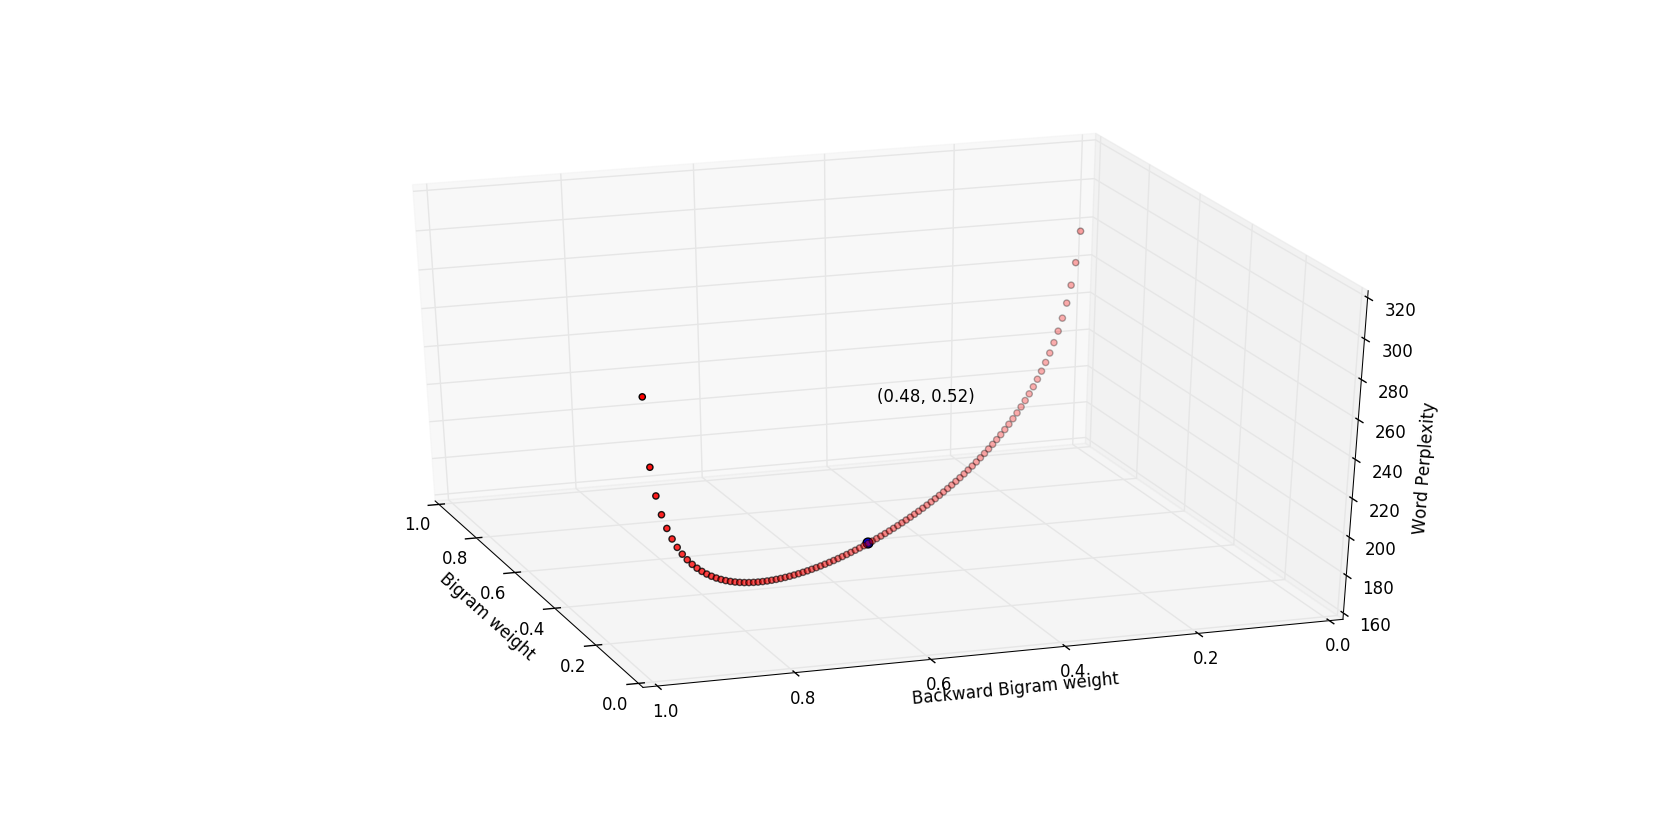
\includegraphics[width=0.8\textwidth]{fig}
\caption{Word perplexity distribution for Bidirectional model on \texttt{Brown} dataset}
\label{fig}
\end{figure}

% --------------------------------------------------------------
%     You don't have to mess with anything below this line.
% --------------------------------------------------------------
\end{document}